\documentclass[x11names]{article}
\usepackage{tikz}
\usepackage{pgfplots}
\usepackage{xcolor}
\usepackage{svg}
\usepackage{amsmath}
\usepackage{array}
\usepackage[skins]{tcolorbox}
\usepackage[version=4]{mhchem}
\usepackage[a4paper, total={6in, 10in}]{geometry}
\usepackage{fourier}
\usepackage{xymtex}
\usepackage{textcomp}
\usepackage{eurosym}
\usepackage{mathrsfs}
\usepackage{float}
\usepackage{pst-all}
\usepackage{pst-3dplot}
\usepackage{leftindex}
\usepackage{verbatim}
\usepackage{import}
\usepackage{xifthen}
\usepackage{pdfpages}
\usepackage{transparent}
\usepackage{import}
\usepackage{pdfpages}
\usepackage{transparent}
\usepackage{amssymb}
\usepackage{mathrsfs}
\usepackage{hyperref}
\usepackage{darkmode}
\usepackage{cancel}

%\enabledarkmode
\definecolor{myblue}{RGB}{224, 245, 255} 
\definecolor{myred}{RGB}{234, 222, 255}
\definecolor{myorange}{RGB}{255, 102, 0}

% box
\newtcolorbox{es}[2][]{%
	enhanced,colback=white,colframe=black,coltitle=black,
	sharp corners,boxrule=0.4pt,
	fonttitle=\itshape,
	attach boxed title to top left={yshift=-0.5\baselineskip-0.4pt,xshift=2mm},
	boxed title style={tile,size=minimal,left=0.5mm,right=0.5mm,
		colback=white,before upper=\strut},
	title=#2,#1
}

% definizioni
\newtcolorbox{blues}[2][]{%
	enhanced,colback=myblue,colframe=black,coltitle=black,
	sharp corners,boxrule=0.4pt,
	attach boxed title to top left={yshift=-0.5\baselineskip-0.4pt,xshift=2mm},
	boxed title style={tile,size=minimal,left=0.5mm,right=0.5mm,
		colback=myblue,before upper=\strut},
	title=#2,#1
}

% teoremi
\newtcolorbox{redes}[2][]{%
	enhanced,colback=myred,colframe=black,coltitle=black,
	sharp corners,boxrule=0.4pt,
	fonttitle=\itshape,
	attach boxed title to top left={yshift=-0.5\baselineskip-0.4pt,xshift=2mm},
	boxed title style={tile,size=minimal,left=0.5mm,right=0.5mm,
		colback=myred,before upper=\strut},
	title=#2,#1
}


% comandi per quadrati dimostrazioni
\newcommand*{\QEDA}{\null\nobreak\hfill\ensuremath{\blacksquare}}%
\newcommand*{\QEDB}{\null\nobreak\hfill\ensuremath{\square}}%

\newcommand{\viola}[1]{\colorbox{myred}{$\displaystyle #1$}}


%% regole
\renewcommand*\contentsname{Indice}
\setcounter{tocdepth}{3}
\setcounter{secnumdepth}{2}
\pgfplotsset{compat=1.15}

\usetikzlibrary{arrows}


\title{Geometria e Algebra lineare}
\author{Federico Cesari}
\date{}



%% DOCUMENTO


\begin{document}
	
\begin{titlepage}
	\begin{center}
		\vspace*{1cm}
		
		\textbf{\LARGE Relazione di laboratorio - Pendolo semplice}
		
		\vspace{0.3cm}
		\large \textit{Misura del periodo di un pendolo semplice} \\
		
		\vspace{0.5cm}
		\Large Federico Cesari \\
		
		\small 1096759 
		\vspace{0.2cm}
		
		\small Gruppo 5
		
		
		\vspace{3cm}
		\begin{center}
			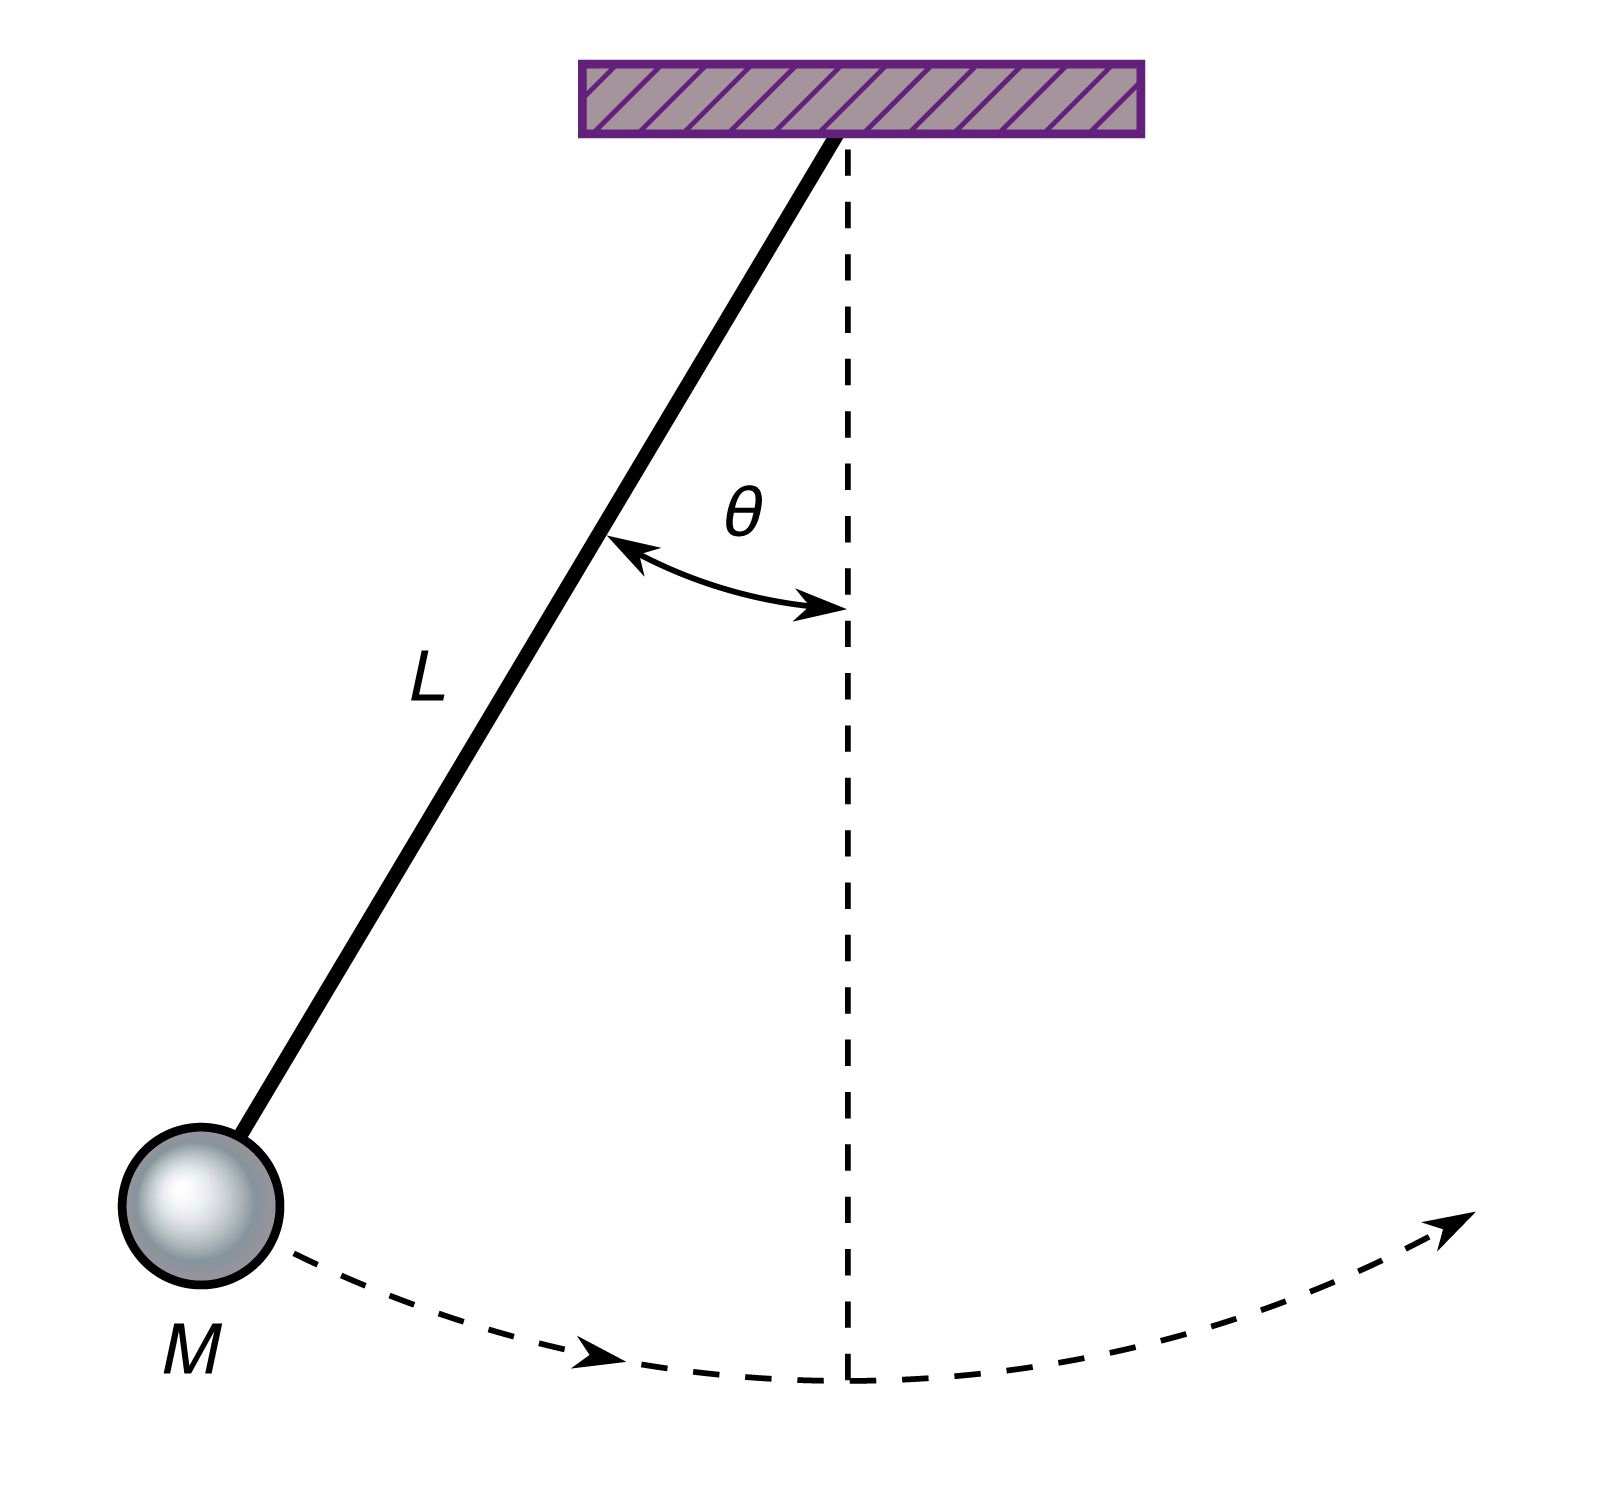
\includegraphics[scale=0.1]{IMG_0200.jpeg}	
		\end{center}
		
		
		
		\vfill
		
		
		
		corso A\\
		Università degli studi di Torino, Torino\\
		4 aprile 2024\\
		
		
	\end{center}
\end{titlepage}
\tableofcontents
\newpage
	
\section{Onde meccaniche}
	Se in casi come il pendolo o un corpo attaccato ad una molla l'oscillazione è \textbf{macroscopica} perché tutto il sistema oscilla, in corpi continui elastici possono prodursi moti oscillatori locali, provocati in una zona specifica del corpo. Questa oscillazione indotta localmente si \textbf{propaga nel mezzo} con una certa velocità costituendo così un'\textbf{onda}.
	
	\begin{center}
		\fboxsep11pt
		\colorbox{myblue}{\begin{minipage}{5.75in}
				\begin{blues}{Definizione: \textbf{Onda}}
					Un'onda è una perturbazione locale impulsiva e periodica che si porpaga in un mezzo (corpo continuo ed elastico) con una certa velocità \(v\). Nel caso unidimensionale parliamo di \textbf{onda piana} \(\xi(x,t)\) la cui deformazione è costante in tutti i punti con stessa \(x\)
				\end{blues}
		\end{minipage}}
	\end{center}
	
	Per descrivere l'andamento di un'onda possiamo: \textbf{fissare un istante \(t\)} e osservare la deformazione su tutto lo spazio \(x\), come se fosse una foto dell'onda; oppure \textbf{fissare un punto dello spazio \(x\)} e osservare al variare del tempo come varia la forma dell'onda, come se fosse un filmato.
	
	\begin{center}
		\textcolor{red}{inserire grafici}
	\end{center}
	
	Vediamo ora come possiamo scrivere l'equazione che descrive la perturbazione in funzione della posizione \(\mathbf{x}\) e del tempo \(\mathbf{t}\): per farlo serviamoci di un sistema di riferimento \(\mathbf{O}\) solidale con l'istante \(t=0\) e un sistema di riferimento \(\mathbf{O'}\) solidale con lo spostamento dell'onda che viaggia a velocità \(v\).
	
	Possiamo quindi descrivere la posizione l'andamento di un'onda piana tramite una funzione del tipo
	
	\[ 
	\begin{cases} 
		x' = x\pm vt \\ \xi' = \xi 
	\end{cases} 
	\quad \Rightarrow \quad \xi(x,t) = \mathbf{f(x \pm vt)}
	\]
	
	Una funzione del tipo \(\mathbf{f(x \pm vt)}\) soddisfa l'equazione differenziale detta \textbf{equazione delle onde} o \textbf{equazione di d'Alembert}:
	
	\[ 
	\nabla^2_\xi- \frac{1}{v^2} \frac{\partial^2\xi}{\partial t^2} = 0 \quad \Rightarrow \quad \boxed{\frac{\partial^2\xi}{\partial x^2} = \frac{1}{v^2}\frac{\partial^2\xi}{\partial t^2}}
	\]
	
	\begin{es}{dimostrazione}
		\[ 
		\mathbf{z = x - vt} \quad \Longleftrightarrow \quad \boxed{\frac{\partial z}{\partial x} = 1}   \quad \quad \boxed{\frac{\partial z}{\partial t} = -v}  \quad \Longleftrightarrow \quad  \mathbf{f = f(z)}
		\]
		
		\[ 
		\textcolor{blue}{\frac{\partial^2 f}{\partial x^2} =} \frac{\partial}{\partial x}\left(\frac{\partial f}{\partial x}\right) =\frac{\partial}{\partial x}\left(\frac{\partial f}{\partial z}\frac{\partial z}{\partial x}\right)  \textcolor{blue}{=\frac{\partial^2 f}{\partial z^2}}
		\]
		\[ 
		\textcolor{red}{\frac{\partial^2 f}{\partial t^2} =} \frac{\partial}{\partial t}\left(\frac{\partial f}{\partial t}\right) =\frac{\partial}{\partial t}\left(\frac{\partial f}{\partial z}\textcolor{orange}{\frac{\partial z}{\partial t}}\right) =\textcolor{cyan}{\frac{\partial}{\partial t}}\left(\textcolor{orange}{-v}\frac{\partial f}{\partial z}\right) = \textcolor{cyan}{-v\frac{\partial }{\partial z}}\left(\textcolor{orange}{-v}\frac{\partial f}{\partial z}\right) \textcolor{red}{=v^2\frac{\partial^2 f}{\partial z^2}}
		\]
		\[ 
	    \frac{\partial^2\xi}{\partial x^2} = \frac{1}{v^2}\frac{\partial^2\xi}{\partial t^2}
		\]
		\newline
		Il passaggio più ambiguo è quello evidenziato in \textcolor{cyan}{ciano}, in cui viene cambiata variabile di derivazione da \(t\) a \(z\). Trattando una funzione qualsiasi, la derivata di qualsiasi funzione rispetto a \(t\) è uguale a \(-v\) derivata rispetto a z (\(-v\) rappresenta il \(dz\) che va a moltiplicare). 
	\end{es}	
	
	\noindent
	Notare che l'equazione delle onde è soddisfatta solo per funzioni che hanno come argomento combinazioni lineari di \(x\) e \(t\) (\(\xi(x \pm vt)\)); è perciò \textbf{l'argomento che importa e non la funzione in sè}. Una combinazione lineare di soluzioni è ancora soluzione dell'equazione, la soluzione generale ha forma
	\[ 
	G(x,t) = f(x-vt) + g(x+vt)
	\]
	


\newpage
\subsection{Onde in una sbarra solida}
	Prendiamo una sbarra solida  e supponiamo di sollecitare  il tratto iniziale applicando una \textbf{forza impulsiva}. Analiziamo un segmento di lunghezza \(dx\): su di esso agiscono la forza elastica \(\vec{F}(x,t)\)  esercitata dagli elementi a sinistra del segmento e la forza elastica \(-\vec{F}(x + dx,t)\) di verso opposto esercitata dagli elementi a destra.

	\begin{center}
		\textcolor{red}{inserire grafici}
	\end{center}
	
	\noindent
	Alla cessazione dello stimolo (\(t'\)) agiscono le forze elastiche e si ha che la lunghezza dell'elemento passa da \(dx\) a 
	\[ 
	(x + dx) + \xi(x+dx,t') \textcolor{gray}{-x - \xi(x,t') } \quad = \quad dx + d\xi
	\]
	Per quanto riguarda le forze invece vale la legge di Hooke secondo la quale
	\[ 
	\textbf{Legge di Hooke} \qquad	F(x) = ES\frac{\partial\xi}{\partial x}
	\]
	Possiamo quindi scrivere la legge del moto con accelerazione \(a = \partial^2 \xi / \partial t^2\):
	\[ 
	\textbf{Risultante} \qquad	dF = \frac{\partial F}{\partial x}dx = \frac{\partial}{\partial x}\left(ES\frac{\partial\xi}{\partial x}\right)dx = ES\frac{\partial^2\xi}{\partial x^2} \mathbf{= dm a} = dm \frac{\partial^2 \xi}{\partial t^2}
	\]
	esprimendo la massa come \(dm = \rho S dx\) si ottiene l'equazione delle onde di d'Alembert dove il coefficiente del termine a destra gioca il ruolo di \(1/v^2\), da questo possiamo scrivere la velocità di propagazione dell'onda:
	\[ 
	E\textcolor{orange}{S}\frac{\partial^2\xi}{\partial x^2}\textcolor{red}{dx} = \rho \textcolor{orange}{S} \textcolor{red}{dx} \frac{\partial^2 \xi}{\partial t^2}
	\]
	
	
	\begin{equation}
		\viola{\frac{\partial^2\xi}{\partial x^2} = \frac{\rho}{E} \frac{\partial^2 \xi}{\partial t^2} \qquad \qquad v = \sqrt{\frac{E}{\rho}}}
	\end{equation}
	
	
	\noindent
	Inoltre oltre allo spostamento \(\xi(x,t)\) si propaga anche la forza \(F(x,t)\). Ciò è verificabile riutilizzando l'epressione della forza nella Legge di Hooke (derivandola prima rispetto a \(t\) e poi rispetto a \(x\)) e ricordando il Teorema di Schwartz, secondo il quale in una derivata mista non dipende dall'ordine di derivazione:
	
	\[ 
	\textcolor{red}{\frac{\partial^2F}{\partial t^2}} = \frac{\partial^2}{\partial t^2} \left(ES\frac{\partial\xi}{\partial x}\right) = \frac{\partial}{\partial x} \left(ES\textcolor{blue}{\frac{\partial^2\xi}{\partial t^2}}\right) = \frac{\partial}{\partial x} \left(ES\textcolor{blue}{v^2\frac{\partial^2\xi}{\partial x^2}}\right) 
	\]
	
	\[ 
	\textcolor{purple}{\frac{\partial^2F}{\partial x^2}} = \frac{\partial^2}{\partial x^2} \left(ES\frac{\partial\xi}{\partial x}\right) = \frac{\partial}{\partial x} \left(ES\frac{\partial^2\xi}{\partial x^2}\right)
	\]
	
	\[ 
	\begin{cases}
		\frac{\partial}{\partial x} \left(ES\frac{\partial^2\xi}{\partial x^2}\right) = \textcolor{purple}{\frac{\partial^2F}{\partial x^2}} \\
		\frac{\partial}{\partial x} \left(ESv^2\frac{\partial^2\xi}{\partial x^2}\right)  =  \textcolor{red}{\frac{\partial^2F}{\partial t^2}}
	\end{cases} \to 
	\begin{cases}
		\frac{\partial}{\partial x} \left(ES\frac{\partial^2\xi}{\partial x^2}\right) = \textcolor{purple}{\frac{\partial^2F}{\partial x^2}} \\
		\frac{\partial}{\partial x} \left(ES\frac{\partial^2\xi}{\partial x^2}\right)  = \frac{1}{v^2} \textcolor{red}{\frac{\partial^2F}{\partial t^2}}
	\end{cases}
	\]
	

	\begin{equation}
		\viola{\frac{\partial^2F}{\partial x^2} = \frac{1}{v^2} \frac{\partial^2 F}{\partial t^2} \qquad \qquad v = \sqrt{\frac{E}{\rho}}}
	\end{equation}

	
	\begin{center}
		\fboxsep11pt
		\colorbox{myblue}{\begin{minipage}{5.75in}
				\begin{blues}{Definizione: onde lognitudinali}
					Quando, come in questo caso, sia lo spostamento \(\xi(x\pm vt)\) sia la forza \(F(x\pm vt)\), campi che descrivono le onde che si propagano lungo l'asse x, sono paralleli alla direzione in cu si propaga la perturbazione, l'onda viene chiamata \textbf{onda longitudinale}.
				\end{blues}
		\end{minipage}}
	\end{center}
	
\newpage
\subsection{Onde in una corda tesa}
	Quando si sposta rapidamente in direzione trasversale l'estremo di una corda tesa (con un estremo fisso) vediamo la perturbazione che si propaga lungo la corda da un estremo all'altro. Supponiamo di spostare leggermente la corda dalla sua posizione di equilibrio e andiamo a studiare le tensioni che agiscono su un segmento di corda \(\mathbf{dl}\). Per piccoli angoli \(\alpha\) e \(\alpha'\) possiamo introdurre le seguenti approssimazioni:
	
	\[ 
	\cos{\alpha} = 1 \quad \cos{\alpha'} = 1 \qquad \qquad \sin{\alpha} = \tan{\alpha} \quad \sin{\alpha'} = \tan{\alpha'}
	\]
	\[ 
	\boxed{\tan\alpha = \frac{\partial \xi}{\partial x} = S(x,t)}
	\]
	
	\begin{center}
		\textcolor{red}{inserire grafici}
	\end{center}
	
	
	\[ 
	dF_x = T(\cos\alpha' - \cos\alpha ) = 0 
	\]
	\[ 
	 dF_y = T(\sin\alpha' - \sin\alpha ) = T(\tan\alpha' - \tan\alpha ) = T\left[S(x+dx,t) - S(x)\right] = TdS = T\frac{\partial S}{\partial x}dx = T\frac{\partial}{\partial x}\left(\frac{\partial \xi}{\partial x}\right)dx = T\frac{\partial^2 \xi}{\partial x^2}dx
	\]
	
	\[ 
	\textbf{Risultante} \qquad	dF =  T\frac{\partial^2 \xi}{\partial x^2}dx  \mathbf{= dm a} = dm \frac{\partial^2 \xi}{\partial t^2} 
	\]
	esprimendo la massa come \(dm = \mu dx\) si ottiene l'equazione delle onde di d'Alembert dove il coefficiente del termine a destra gioca il ruolo di \(1/v^2\), da questo possiamo scrivere la velocità di propagazione dell'onda:
	\[ 
	T\frac{\partial^2\xi}{\partial x^2}\textcolor{red}{dx} = \mu \textcolor{red}{dx} \frac{\partial^2 \xi}{\partial t^2}
	\]

	\begin{equation}
		\viola{	\frac{\partial^2\xi}{\partial x^2} = \frac{\mu}{T} \frac{\partial^2 \xi}{\partial t^2} \qquad \qquad v = \sqrt{\frac{T}{\mu}}}
	\end{equation}
	
	\begin{center}
		\fboxsep11pt
		\colorbox{myblue}{\begin{minipage}{5.75in}
				\begin{blues}{Definizione: onde trasversali}
					Quando, come in questo caso, le particelle del mezzo attraversato subiscono spostamenti in direzione perpendicolare alla direzione in cui si propaga l'onda l'onda viene chiamata \textbf{onda trasversale}.
				\end{blues}
		\end{minipage}}
	\end{center}
	
\newpage
\subsection{Onde nei gas}
	Se per i solidi la deformazione dipende dal modulo di Young secondo la legge \(\frac{\Delta L}{L} = \frac{1}{E}\sigma\), nel caso dei gas la variazione relativa di volume segue la legge
	\[ 
	\frac{\Delta V}{V} = -\frac{1}{\beta} \Delta p
	\] \\
	
	\noindent
	Supponiamo di avere del gas imperturbato (\(\rho_0, p_0\)) bloccato da due pistoni. Fornendo un impulso di pressione tramite i pistoni provociamo una compressione adiacente con una \textbf{conseguenti variazione di densità di massa}.
	
	\[
	\rho = \rho + d\rho \qquad p = p_0 + dp
	\]
	
	\subsubsection{Densità}
	Considero un elemnto di gas di massa \(dm = \rho_0S(dx)\) che a seguito della perturbazione subisce uno spostamento che lo porta a stare tra
	\[
	x + \xi(x,t') \quad \text{ e } \quad x + dx + \xi(x + dx,t')
	\]
	Così la sua dimensione diventa
	\[
	x + dx + \xi(x + dx,t') \textcolor{gray}{-x - \xi(x,t')} = dx + \xi(x + dx,t')- \xi(x,t') = dx + \frac{\partial \xi}{\partial x}dx = dx\left(1 + \frac{\partial \xi}{\partial x}\right)
	\]
	A partire da questa nuova espressione della "larghezza" dell'elemnto infinitesimo posso scrivere l'espressione della densità dopo la compressione:
	\[
	\rho = \frac{dm}{dV} = \frac{dm}{S(dx)} \frac{\rho_0 \textcolor{red}{S (dx)}}{\textcolor{red}{S(dx)}\left(1 + \frac{\partial \xi}{\partial x}\right)} = \rho_0\left(1 + \frac{\partial \xi}{\partial x}\right)^{-1}
	\]
	Ora andremo ad applicare una semplificazione bizzarra. Se la deformazione specifica $|\varepsilon| = \left|\frac{\partial \xi}{\partial x}\right|<< 1$, allora si può applicare la formula del binomio:
	\[
	\left(1 + \varepsilon\right)^{-n} = 1 - n\varepsilon + \textcolor{gray}{\frac{n(n+1)}{2!}\varepsilon^2\dots}
	\]
	Quindi posso scrivere la densità come
	\[
	\rho \approx \rho_0\left(1 - \frac{\partial \xi}{\partial x}\right)
	\]
	da cui la variazione
	\begin{equation} \label{rho}
	d\rho(x,t) = \rho - \rho_0 = - \rho_0\frac{\partial \xi}{\partial x}
	\end{equation}
	in cui il segno meno indica ce se il volumetto è compresso la densità aumenta, mentre se si espande la densità diminuisce.
	
	\subsubsection{Pressione}
	Ad una variazione di densità corrisponde una variazione di pressione secondo la legge
	\[
	\beta = \rho\frac{dp}{d\rho} \quad \to \quad dp(x,t) = p(x,t) - p_0 = \beta\frac{d\rho}{\rho}
	\]
	da cui derivo che la pressione è 
	\[
	p(x,t) = \beta\frac{d\rho}{\rho_0} +  p_0 
	\]
	Sostituendo l'espressione della densità trovata prima nella \ref{rho} scrivo
	\[
	p(x,t) = \beta\frac{- \rho_0\frac{\partial \xi}{\partial x}}{\rho_0} +  p_0 =p_0 - \beta\frac{\partial \xi}{\partial x}
	\]
	\subsubsection{Forza}
	La variazione di pressione causa un movimento del gas e la risultante su $dm$ è 
	\begin{align*}
	-dF = F(x,t') - F(x+dx.t') =& S\left[p(x,t') - p(x+dx,t')\right] \\
							   =& S(dp) \\
							   =& -S\frac{\partial p}{\partial x}dx \\
							   =& -S\frac{\partial}{\partial x}\left(p_0 - \beta\frac{\partial \xi}{\partial x}\right)dx \\
							   =& S\beta\frac{\partial^2\xi}{\partial x^2}dx
	\end{align*}
	
	\[ 
	\textbf{Risultante} \qquad	-dF = S\beta\frac{\partial^2\xi}{\partial x^2}dx  \mathbf{= dm a} = \rho_0 S(dx) \frac{\partial^2 \xi}{\partial t^2} 
	\]
	
	\begin{equation} \label{gas}
		\viola{\frac{\partial^2\xi}{\partial x^2} = \frac{\rho_0}{\beta} \frac{\partial^2 \xi}{\partial t^2} \qquad \qquad v = \sqrt{\frac{\beta}{\rho_0}}}
	\end{equation}
	
	Lungo la colonna di gas si propagano anche un'onda i pressione e una perturbazione di densità del gas, tuttue con la stessa velocitù data da \ref{gas}.
	
	\subsubsection{Modulo di compressibilità adiabatica}
	Nel caso di trasformazioni adiabatiche vale (come dimostreremo più avanti) l'uguaglianza
	\[
	pV^\lambda = \text{costante}
	\]
	dalla quale, sviluppando il differenziale si possono trovare alcune caratteristiche di \(\beta\) in condizioni adiabatiche:
	\[
	d\left(pV^\gamma\right) = V^\gamma (dp) + \gamma p V^{(\gamma - 1)}dV \boldsymbol{= 0}
	\]
	\[ 
	\to \quad  V^\gamma (dp) = \gamma p V^{(\gamma - 1)}(dV) \quad \to \quad \frac{\textcolor{red}{V^\gamma} (dp)}{p\textcolor{red}{V^\gamma}} = \frac{\gamma \textcolor{red}{p} V^{(\gamma - 1)}(dV)}{\textcolor{red}{p}V^\gamma}
	\]
	Dalla quale otteniamo (confrontata con l'espressione precedente di \(\beta\))
	\[ 
	\frac{dp}{p} = \gamma\frac{dV}{V} 
	\]
	\[ 
	\frac{dV}{V} = \frac{1}{p\gamma}dp  \qquad \qquad \frac{\Delta V}{V} = -\frac{1}{\beta} \Delta p
	\]
	Da cui si ottiene la nuova espressione di \(\beta\)
	
	
	\begin{equation}
		\viola{\beta = \gamma p}
	\end{equation}
	
	\begin{es}{calcolo velocità del suono}
		Se assimiliamo l'aria ad un gas perfetto biatomico (\(\gamma = 7/5\)) dai risultati ottenuti fin'ora si trova che:
		\[ 
		v = \sqrt{\frac{\beta}{\rho_0}} = \sqrt{\frac{\gamma p_0}{\rho_0}} = \sqrt{\frac{(7/5)\cdot 1.01325\cdot 10^5}{1.29}} = 331.6 \frac{m}{s}
		\]
		Il risultato ottenuto è in accordo (3\%) con quello misurato, possiamo quindi dedurre che l'aprossimazione adiabatica è una bona approssimazione.
	\end{es}
	
	
\newpage
\section{Onde piane armoniche}
Un tipo molto importante di onda piana è l'\textbf{onda armonica} la cui forma si scrive

\[ 
\xi(x,t) = \xi_0 \sin\left(\boldsymbol{k}x \mp \boldsymbol{\omega} t + \boldsymbol{\delta}\right)
\]
dove \(k\) è il \textbf{numero d'onde}.
\begin{center}
	\textcolor{red}{inserire grafici}
\end{center}

\noindent
\paragraph{Periodo spaziale} Fissato un tempo \(t=t_0\), definiamo la lunghezza d'onda \(\lambda\) come la periodicità spaziale dell'onda. Essendo \(\lambda\) lo spazio tra due creste d'onda possiamo calcolarla come \(\lambda = x_2 - x_1 = 2\pi / k\), da cui si deduce che \(k\) è uguale al numero di lunghezze d'onda in un intervallo spaziale pari a \(2\pi\) metri.

In generale il periodo spaziale può essere espresso tramite \(\lambda\) o \(k\).

\begin{center}
	\fboxsep11pt
	\colorbox{myblue}{\begin{minipage}{5.75in}
			\begin{blues}{Lunghezza d'onda \(\lambda\)}
				La lungheza d'onda è lo spazio percorso dalla perturbaione nell'intervallo di tempo di un periodo \(T\).
				\[ 
				\lambda = \frac{2\pi}{k} = vT
				\]
			\end{blues}
	\end{minipage}}
\end{center}

\paragraph{Periodo temporale} Fissato unpunto nello spazio \(x=x_0\), definiamo il periodo \(T = t_2-t_2\)

\[ T = \frac{2\pi}{\omega}\] 
come l'intervallo temporale tra due istanti nei quali l'onda, essendo armonica, assume lo stesso valore.

Sapendo che la pulsazione è la velocità dell'onda nel percorrere un giro (\(2\pi\)), i due periodi dono legati dalla relazione
\[ 
\lambda = vT
\]
Quindi possiamo esprimere il periodo temporale tramite \(T\), \(f\), \(\omega\).\\

\noindent
Tutte le espressioni della funzione d'onda sono:

\[ 
\xi(x,t) = \xi_0 \sin\left(kx \mp \omega t + \delta\right) \qquad \xi(x,t) = \xi_0 \sin\left[ 2\pi\left(\frac{x}{\lambda} \mp \frac{t}{T}\right) + \delta\right]  \qquad \xi_0\sin\left[\frac{2\pi}{\lambda}\left(x \mp vt\right) + \delta \right]
\]
	\newpage
	\subsection{Analisi di Fourier}
	\subsection{Onde sulla superficie di un liquido}
	
	
	\newpage
	\subsection{Propagazione dell'energia in una barra solida}
	La propagazione di un campo che descrive in'onda è sempre accompagnato da una propagazione di energia. Osserviamo prima il fenomeno del flusso di energia legato alla propagazione di un'onda piana armonica in una barra solida andando a calcolare la potenzia media e l'energia per untià di volume ad essa associata.\\
	
	\begin{center}
		\textcolor{red}{inserire grafici}
	\end{center}
	
	\noindent
	Per prima cosa mettiamo in evidenza le equazioni che entrano in gioco:
	\[ 
	\textbf{Onda:} \quad \xi(x,t) = \xi_0\sin\left(kx - \omega t\right)
	\]
	\[ 
	\textbf{Forza:} \quad F = -ES\frac{\partial\xi}{\partial x}
	\]
	L'espressione della potenza è 
	
	\begin{align*}
		\mathcal{P} =& \vec{F} \cdot \vec{u} \\
					=& -ES\frac{\partial\xi}{\partial x}\frac{\partial\xi}{\partial t} \\
					=& -ES\left[k\xi_0\cos\left(kx -\omega t\right)\right]\left[-\omega \xi_0\cos\left(kx -\omega t\right)\right] \\
					=& ESk\omega \xi_0^2\cos^2\left(kx-\omega t\right)
	\end{align*}
	La potenza quindi è una cosinusoide traslata in alto di una sua ampiezza (con avvallamenti tangenti all'asse orizzontale). la potenza media è espirmibile come la retta che interseca la cosinusoide alla quota pari a metà la sua ampiezza; poi ricordandoci che
	
	\[ 
	\boxed{v = \sqrt{E/\rho} \qquad E = v^2 \rho} \qquad \boxed{k = \frac{\omega}{v}}
	\]
	
	\begin{align*}
		\mathcal{P}_m =& \frac{1}{2} ESk\omega \xi_0^2  \\
			=& \frac{1}{2} (v^2 \rho)S\left(\frac{\omega}{v}\right) \omega\xi_0^2 
	\end{align*}
	
	\begin{equation}
		\viola{\mathcal{P}_m = \frac{1}{2}\rho \omega^2 \xi^2 S v}
	\end{equation}
	
	
	\subsubsection{Energia per unità di volume}
	Considero l'elemento infinitesimo di massa \(dm = \rho dV = \rho S dx\) descrive un moto armonico con 
	\[ 
	\textbf{Posizione:} \quad \xi(x,t) = \xi_0\sin\left(kx - \omega t\right) 
	\]
	\[ 
	\textbf{Velocità} \quad v(x,t)= \frac{\partial\xi}{\partial t} = \omega \xi_0\cos\left(kx - \omega t\right) 
	\]
	Quindi l'energia meccanica risulta pari all'energia cinetica massima assunto dall'elemento \(dm\), che si trova utilizzando la velocità massima \(v_{\text{max}} = \omega \xi_0\):
	
	\[ 
	dU = \frac{1}{2}(dm)v_{\text{max}}^2 = \frac{1}{2}\rho S (dx)\omega^2 \xi_0^2 = \frac{1}{2}\rho (dV)\omega^2 \xi_0^2
	\]
	Chiamiamo \textbf{densità di energia per unità di volume} il valore 
	\[
	\mathcal{W} = \frac{dU}{dV} = \frac{1}{2}\rho \omega^2\xi_0^2
	\]
	con la quale possiamo esprimere la potenza media come 
	
	\begin{equation}
		\viola{\mathcal{P}_m = \mathcal{W}S v}
	\end{equation}

	
	\subsubsection{Intensità dell'onda}
	Definiamo l'intensità di un'onda come  \textbf{potenza media per unità di superficie}, quindi
	
	\[
	I = \frac{\mathcal{P}}{S} = \frac{1}{2}\rho\omega^2\xi_0^2v
	\]
	
	\subsection{Propagazione dell'energia in una corda tesa}
	Studiamo ora lo stesso fenomeno ma in una corda tesa. La situazione è simile con la differenza che l'onda ora è trasversale.
	
	\begin{center}
		\textcolor{red}{inserire grafici}
	\end{center}
	
	\noindent
	Per prima cosa mettiamo in evidenza le equazioni che entrano in gioco:
	\[ 
	\textbf{Onda:} \quad \xi(x,t) = \xi_0\sin\left(kx - \omega t\right)
	\]
	\[ 
	\textbf{Forza:} \quad F = T
	\]
	L'espressione della potenza è 
	
	\begin{align*}
		\mathcal{P} =& \vec{F} \cdot \vec{u} \\
		=& T\frac{\partial\xi}{\partial t}\cos{\left(\frac{\pi}{2} + \alpha\right)} \qquad  \cos{\left(\frac{\pi}{2} + \alpha\right)} = \sin{\alpha} \approx \tan\alpha = \frac{\partial\xi}{\partial x} \\
		= & T\frac{\partial\xi}{\partial t}\frac{\partial\xi}{\partial x} \\
		=& Tk\omega \xi_0^2\cos^2\left(kx-\omega t\right)
	\end{align*}
	Trovo la potenza media come prima esprimendo \(k\) e \(T\) come
	\[ 
	\boxed{v = \sqrt{T/\mu} \qquad T = v^2 \mu} \qquad \boxed{k = \frac{\omega}{v}}
	\]
	
	\begin{equation}
		\viola{\mathcal{P}_m = \frac{1}{2}\mu\omega^2\xi^2v}
	\end{equation}
	
	
	\subsubsection{Energia per unità di lunghezza}
	Considero l'elemento infinitesimo di massa \(dm = \mu dx \) descrive un moto armonico con 
	\[ 
	\textbf{Posizione:} \quad \xi(x,t) = \xi_0\sin\left(kx - \omega t\right) 
	\]
	\[ 
	\textbf{Velocità} \quad v(x,t)= \frac{\partial\xi}{\partial t} = \omega \xi_0\cos\left(kx - \omega t\right) 
	\]
	Quindi l'energia meccanica risulta pari all'energia cinetica massima assunto dall'elemento \(dm\), che si trova utilizzando la velocità massima \(v_{\text{max}} = \omega \xi_0\):
	
	\[ 
	dU = \frac{1}{2}(dm)v_{\text{max}}^2 = \frac{1}{2}\mu(dx)\omega^2 \xi_0^2 
	\]
	Chiamiamo \textbf{densità di energia per unità di lunghezza} il valore 
	\[
	\mathcal{W} = \frac{dU}{dx} = \frac{1}{2}\mu \omega^2\xi_0^2
	\]
	con la quale possiamo esprimere la potenza media come 
	
	\begin{equation}
		\viola{\mathcal{P}_m = \mathcal{W} v}
	\end{equation}

	
	
	
	
	\newpage
	\subsection{Onde in più dimensioni}	
	Prima di tutto definiamo \textbf{fronte d'onda} la superfici su cui in un certo istante la fase dell'onda è costante (\(\phi = kx -\omega t\)). 

	Per le onde piane il fronte d'onda è un piano che si sposta con velocità \(v\) dell'onda. Per caratterizzare la direzione di propagazione dell'onda introduciamo il \textbf{vettore di propagazione} \(\vec{k}\) con \(k = 2\pi/\lambda\) e verso uguale a quello di \(\vec{v}\) e il vettore posizione \(\vec{r}\) che individua la posizione di un punto P su un certo fronte d'onda. Con queste informazioni possiamo riscrivere la funzione d'onda come
	\[ 
	\xi(r,t) = \xi_0 \sin\left(\vec{k}\cdot \vec{r}- \omega t\right) 
	\]
	In un sistema di tre coordinate l'equazione generale delle onde ammette altre soluzioni che rappresentano \textbf{onde sferiche} e \textbf{onde cilindriche}: 
	\[ 
	\nabla^2\xi (x,y,z,t) = \frac{1}{v^2}\frac{\partial^2\xi (x,y,z,t)}{\partial t^2}
	\]
	\subsubsection{Onde elastiche in una membrana tesa}
	Consideriamo una membrana piana tesa con tensione \(T\). Supponiamo di spostare leggermente la membrana dalla sua posizione di equilibrio e andiamo a studioare le tensioni che agiscono su un'area \(dxdy\). 
	
	Il ragionamento è uguale a quello fatto per la corda tesa, in questo caso però la tensione si distribuisce su tutto il lato \(d*\) e diventa \(T(d*)\):
	
	\begin{center}
		\textcolor{red}{inserire grafici}
	\end{center}
	
	\[ 
	dF_x(x,y,z,t) = T(dx)\frac{\partial^2 \xi(x,y,t)}{\partial y^2}dy = T\frac{\partial^2\xi(x,y,t)}{\partial y^2}dxdy
	\]
	\[ 
	dF_y(x,y,z,t) = T\frac{\partial^2 \xi(x,y,t)}{\partial x^2}dx = T(dy)\frac{\partial^2\xi(x,y,t)}{\partial x^2}dxdy 
	\]
	
	\[ 
	\textbf{Risultante} \qquad	dF = T\left(\frac{\partial^2\xi(x,y,t)}{\partial y^2} + \frac{\partial^2\xi(x,y,t)}{\partial x^2}\right)dxdy \mathbf{=(dm)a = }  \rho_s(dxdy)\frac{\partial^2\xi(x,y,t)}{\partial t^2}
	\]
	esprimendo la massa come \(dm = \rho_s (dxdy)\) si ottiene l'equazione delle onde di d'Alembert dove il coefficiente del termine a destra gioca il ruolo di \(1/v^2\), da questo possiamo scrivere la velocità di propagazione dell'onda:
	
	\[ 
	T\left(\frac{\partial^2\xi(x,y,t)}{\partial y^2} + \frac{\partial^2\xi(x,y,t)}{\partial x^2}\right)\textcolor{red}{dxdy} = \rho_s(\textcolor{red}{dxdy})\frac{\partial^2\xi(x,y,t)}{\partial t^2}
	\]
	
	
	\begin{equation}
		\viola{\frac{\partial^2\xi(x,y,t)}{\partial y^2} + \frac{\partial^2\xi(x,y,t)}{\partial x^2} = \frac{\rho_s}{T}\frac{\partial^2\xi(x,y,t)}{\partial t^2} \qquad v = \sqrt{\frac{T}{\rho_s}}}
	\end{equation}

	
	
	
	\subsubsection{Onde sferiche}
	Se il mezzo è \textit{isotropo} è quindi la velocità di propagazione è uguale in tutte le direzioni, la funzoine d'\textbf{onda sferica armonica} è \(\xi(r,t) = A(r)\sin\left(kr -\omega t\right)\) dove \(r\) è la distanza dalla sorgfente e \(A(r)\) è l'ampiezza funzione di \(r\). \\
	
	\noindent
	Diciamo che la nostra sorgente emetta un'onda di intensità \(I(r) = CA^2(r)\) dove \(C\) è una costante dipendente dal mezzo. In un'onda sferica la \textbf{potenza media} trasmessa attraverso la superficie sferica \(S = 4\pi r^2\) deve risultare \textbf{costante} ad ogni valore di \(r\):
	
	\[ 
	\mathcal{P}_m = \textcolor{blue}{I}S = \text{cost.}
	\] 
	
	\[ 
	\mathcal{P}_m = \textcolor{blue}{CA^2}4\pi r^2 = \text{cost.}
	\]
	
	\[ 
	A(r) = \sqrt{\frac{\mathcal{P}_m}{4\pi r^2}} = \frac{1}{2r}\sqrt{\frac{\mathcal{P}_m}{\pi}}
	\]

	\noindent
	Risulta quindi che l'ampiezza è inversamente proporzionale alla distanza \(r\), come la pressione, e quindi può essere scritta come \(A = \xi_0 /r\).
	\begin{equation}
		\viola{\xi(r,t) = \frac{\xi_0}{r}\sin\left(kr -\omega t\right)}
	\end{equation}
	mentre l'intensità è inversamente proporzionale al quadrato della distanza dalla sorgente:
	
	\[ 
	I(r) = \frac{\mathcal{P}_m}{S} = <
	\]
	
	\begin{center}
		\textcolor{red}{PERCHE SI TRATTA COME UNA CORDA?????????}
	\end{center}
	
	\subsection{Onde cilindriche}
	


	\newpage
	\subsection{Assorbimento dell'energia}
	Come abbiamo visto l'intensità di un'onda non rimane costante ma decresce al propagarsi dell'onda (nelle onde sferiche più rapidamente, nelle cilindriche meno...). Questo comportamento viene attribuito ad un \textbf{assorbimento di energia} dovuto a fenomeni di attrito interno. Studiando il fenomeno su uno spessore \(dx\) si ha un'aattenuazione che può essere considerata proporzionale all'intensità in \(x\) e allo spessore \(dx\).
	
	\[ 
 	dI = -\boldsymbol{\alpha} I(x)dx
	\]
	
	dove \(\alpha\) è il \textbf{coefficiente di assorbimento}.
	
	\[ 
	\int_{I_0}^{I} \frac{dI}{I} = -\alpha\int_{0}^{x} dx 
	\]
	\begin{equation}
 		\viola{I(x) = I_0e^{-\alpha x}}
	\end{equation}
	Quindi la decrescità dell'intensità è esponenziale. Definiamo la distanza \(x_0 = \frac{1}{\alpha}\) detta \textbf{lunghezza di assorbimento} la distanza tra due punti tali che \(I(x_1)/I(x_2) = \frac{1}{e}\).\\
	
	\noindent
	Abbiamo appurato precedentemente che l'ampiezza dell'onda è direttamente proporzionale a \(\sqrt{I}\)
	
	\[ 
	I = CA^2 \quad \to \quad A = \sqrt{\frac{I}{C}} = \sqrt{\frac{I_0e^{-\alpha x}}{C}}
	\]
	quindi la funzione d'onda in un mezzo che assorbe energia è:
	
	\[ 
	\textbf{Onde piane:}\qquad \xi = \left(\frac{I_0e^{-\alpha x}}{C}\right)^{\frac{1}{2}} \sin\left(kx-\omega t\right) \quad = \quad \xi_0 \left(I_0e^{-\alpha x/2}\right)^{\frac{1}{2}}\sin\left(kx-\omega t\right)
	\]
	\[ 
	\textbf{Onde sferiche:}\qquad \xi = \frac{\left(\frac{I_0e^{-\alpha x}}{C}\right)^{\frac{1}{2}}}{r} \sin\left(kx-\omega t\right) \quad = \quad \xi_0 \frac{\left(I_0e^{-\alpha x/2}\right)^{\frac{1}{2}}}{r}\sin\left(kx-\omega t\right)
	\]
	\[ 
	\textbf{Onde cilindriche:}\qquad \xi = \frac{\left(\frac{I_0e^{-\alpha x}}{C}\right)^{\frac{1}{2}}}{\sqrt{r}} \sin\left(kx-\omega t\right) \quad = \quad \xi_0 \frac{\left(I_0e^{-\alpha x/2}\right)^{\frac{1}{2}}}{\sqrt{r}}\sin\left(kx-\omega t\right)
	\]
	
	\newpage
	\subsection{Pacchetti d'onde}
	Fino ad ora abbiamo considerato onde armoniche di lunghezza e durata infinita. Tutte le sorgenti emettono onde attraverso processi di durata finita, quindi, nella realtà, un'onda ha una propria durata e estensione spaziale.\\
	
	\noindent
	Considerato un pacchetto di lughezza \(\Delta x\) e durata \(\Delta t\), tali che \(\Delta x = v\Delta t\). Il pacchetto è poi caratterizzato da \(N\) oscillazioni tali che
	
	\[ 
\Delta x  =N \lambda \qquad \Delta t = NT 
	\]
	ed esprimiamo il numero di onde \(k\) e la pulsazione \(\omega\) come
	
	\[ 
	k = \frac{2\pi}{\lambda}= \frac{2\pi N}{\Delta x} \qquad \omega = \frac{2\pi}{T} = \frac{2\pi N}{\Delta t}
	\]
	
	\begin{center}
		\textcolor{red}{inserire grafici}
	\end{center}
	Se ammettiamo (come nella figura) che N non sia fisso ma abbia una acerta indeterminazione che esprimiamo come \(\Delta N = 1\), possiamo trovare altre espressioni per \(k\) e \(\omega\):
	
	\[ 
	\boxed{\Delta k = \frac{2\pi}{\Delta x}} \qquad \boxed{ \Delta\omega = \frac{2\pi}{\Delta t}} \qquad \boxed{\Delta f = \frac{1}{\Delta t}}
	\]
	
	\[ 
	\viola{\Delta k \Delta x = 2\pi} \qquad \viola{\Delta \omega \Delta t = 2\pi} \qquad \viola{\Delta f \Delta t = 1}
	\]
	Queste osservazioni mettono i vevidenza la sostanziale differenza tra onda e pacchetto d'onda: mentre la prima ha una lunghezza d'onda \(\lambda\)  e una frequenza \(f\) ben definite che la descrivono completamente, nel secondo è presente una \textbf{banda di frequenze} e un \textbf{intervallo di numeri d'onda}
	\[ 
	\Delta f = \frac{1}{\boldsymbol{\Delta t}} \qquad \Delta k = \frac{2\pi}{\boldsymbol{\Delta x}}
	\]
	Da quest'ultime espressioni notiamo che al crescere di \(\Delta x\) e \(\Delta t\) minori risultano queste bande, infatti la limite per \(\Delta x,\Delta t \to \infty\) troviamo l'onda armonica. Se andiamo a considerare \textbf{brevi durate e piccole lunghezze} nel pacchetto sono contenute bande di lunghezze d'onda e frequenze distribuite significatibamente nell'intorno di \(\lambda\) \(f\).
	
		\subsubsection{Velocità di fase e velocità di gruppo}
		Poiché diversi segmenti d'onda contenuti in un pacchetto possono avere frequenze diverse, la velocità del pacchetto non può essere identificata con quella delle componenti. Tuttavia è essenziale identificare la velocità del pacchetto perché il fenomeno fisico è rappresentato proprio dal pacchetto ed è la sua velocità quella con cui si propaga l'\textbf{energia} dell'onda.     
		
		Andiamo quindi a distinguere la \textbf{velocità di fase}, quella con cui si muovono le singole componenti dell'onda, e \textbf{velocità di gruppo}. 
		La velocità dell'onda dipende dalla frequenza quando la propagazione avviene in un \textbf{mezzo dispersivo} come può avvenire per onde sulla superficie di un liquido o onde elettromagnetiche in mezzi materiali o in cavità conduttrici.\\
		
		\noindent
		Mostriamo un esempio di velocità di gruppo nel caso di un pacchetto con solo due onde armoniche:
		
		\[ 
		\xi(x,t) = \xi_0\sin\left(k_1x -\omega_1 t\right) + \xi_0\sin\left(k_2x -\omega_2 t\right)
		\]
		\[ 
		\textcolor{gray}{\textit{prostaferesi: } \quad \sin\alpha + \sin\beta = 2\sin\left(\frac{\alpha + \beta}{2}\right)\cos\left(\frac{\alpha - \beta}{2}\right)}
		\]
		\[ 
		\xi(x,t) = 2\xi_0\sin\left(\frac{(k_1 + k_2)x - (\omega_1 + \omega_2)t}{2}\right) \cos\left(\frac{(k_1 - k_2)x + (\omega_2 - \omega_1)t}{2}\right)
		\]
		Definiti \(k_m,\omega _m\) e \(\Delta k,\Delta\omega\)
		\[ 
		\boxed{k_m = \frac{k_1 + k_2}{2}} \qquad \boxed{\omega _m = \frac{\omega _1 + \omega _2}{2}} \qquad \boxed{\Delta k=\frac{k_1 - k_2}{2}} \qquad \boxed{\Delta \omega = \frac{\omega_1 - \omega_2}{2}}
		\]
		\[ 
		\viola{\xi(x,t) = 2\xi_0\cos\left(\frac{\Delta k}{2}x - \frac{\Delta\omega}{2}t \right)\sin\left(k_mx - \omega_mt\right)}
		\]
		\begin{center}
			\textcolor{red}{inserire grafici}
		\end{center}
		
		
		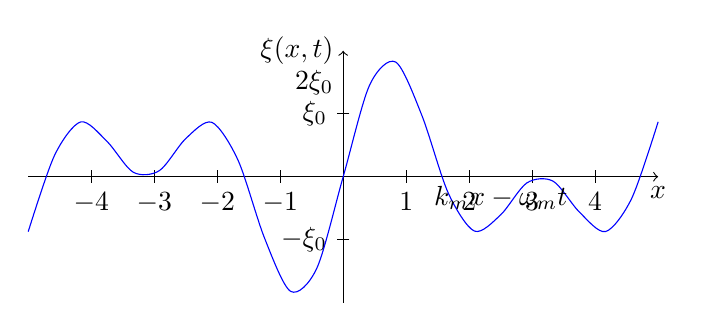
\begin{tikzpicture}[scale=0.8]
			% Assi cartesiani
			\draw[->] (-5,0) -- (5,0) node[below] {$x$};
			\draw[->] (0,-2) -- (0,2) node[left] {$\xi(x,t)$};
			% Etichette sugli assi
			\foreach \x/\xtext in {-4/-4, -3/-3, -2/-2, -1/-1, 1/1, 2/2, 3/3, 4/4}
			\draw (\x,0.1) -- (\x,-0.1) node[below] {$\xtext$};
			\foreach \y/\ytext in {-1/-\xi_0, 1/\xi_0}
			\draw (0.1,\y) -- (-0.1,\y) node[left] {$\ytext$};
			% Grafico
			\draw[domain=-5:5, smooth, variable=\x, blue] plot ({\x},{2*cos(deg(0.5*\x)) * sin(deg(2*\x))});
			% Etichette
			\node[below] at (2.5,0) {$k_m x - \omega_m t$};
			\node[left] at (0,1.5) {$2\xi_0$};
		\end{tikzpicture}
		
		
	
		In sostanza il moto relativo di un'onda rispetto all'altra produce la sovrapposizione mostrata sopra: \textbf{l'onda di alta frequenza cambia} durante il moto ma \textbf{l'inviluppo conserva la stessa forma}.
		
		L'ampiezza dell'onda modulata
		\[ 
		A = 2\xi_0\cos\left(\frac{\Delta k}{2}x - \frac{\Delta\omega}{2}t \right)
		\]
		non è costante ma presenta una struttura di tipo ondulatorio e descrive l'inviluppo dell'onda di alta frequenza.
		
		Abbiamo quindi un'onda di alta frequenza che si propaga con velocità di fase \(v_f\) e con ampiezza modulata da un'onda che si propaga con velocità \(v_g\) velocità di gruppo:
		\[ 
		\boldsymbol{v_f} = \frac{\omega _m}{k_m} \qquad \boldsymbol{v_g} = \frac{\Delta \omega }{\Delta k}
		\]
		              
	
	\newpage
	\subsection{Effetto Doppler}
	\subsection{Onda d'urto}
	
	\newpage
	\section{Onde stazionarie}
	Un'altro tipo di oscellazioni rilevanti sono le onde stazionarie. Per semplicità andremo a considerare onde su una corda fissata ai due estremi. Si osserva che le posizioni di massima ampiezza e dei punti fermi (nodi) non variano nel tempoo. Possiamo quindi definire questo tipo di oscillazione un'\textbf{oscillazione collettiva} del fenomeno \textbf{cui non è associato un fenomeno di propagazione}. \\
	
	\noindent
	Consideriamo una corda fissa ad un solo estremo; sull'estremo libero applichiamo una perturbazione \textbf{sinusoidale} regressiva di frequenza \(f\) tramite un diapason:
	\[ 
	\xi_1 (x,t) = A\sin\left(kx +\omega t\right) 
	\]

\newpage
\section{Fluidi}
	
	
	
\end{document}




